\newpage
\section{Traffic Distributions via Feynman Diagrams}
\label{sec:feynman-physics}

One of our motivations is to connect graph polynomials with the celebrated Feynman diagram technique from physics.
In quantum field theory, Feynman diagram expansion is used to reduce matrix integrals into graphical calculations.
We show in this section that this method can (heuristically) derive the traffic distribution of orthogonally invariant distributions (\cref{thm:moments}).

The matrix model that we consider in this section is specified by a {\em potential
function} $V:\R\to\R$, and has partition function
\begin{equation}\label{eq:action}
    Z \defeq \int_{\mathcal M}\d\bA\ e^{-\frac n2\Tr V(\bA)}\,,
\end{equation}
where $\mathcal M \defeq \R^{n\times n}_{\sym}$ is the space of symmetric $n\times n$
matrices. Equivalently, this is the partition function of the random matrix
$\bA\in\mathcal M$ sampled from the probability measure
$\mu_V(\bA)\propto \exp(-\frac n2\Tr V(\bA))$, which is a special case of an
orthogonally invariant distribution (\cref{sec:rot-inv}).

In physics, matrix integrals such as~\cref{eq:action} are viewed as a
$0$-dimensional theory: the variable is a matrix, and the partition
function is a finite-dimensional integral rather than a functional integral over
fields on space-time. The large-$n$ expansion of such integrals is organized into diagrammatic
contributions indexed by {\em Feynman diagrams}.
\begin{enumerate}
    \item In the limit $n\to\infty$, only planar diagrams contribute at leading
    order, an observation going back to foundational work of 't~Hooft~\cite{tHooft1974planar, brezin1978planar}. Related planarity phenomena also appear in
    mathematics, for example in the connections between large random matrices and
    non-crossing pairings.

    \item In special scaling limits of the potential
    with $n$, the Feynman diagram expansion can be interpreted in terms of physical theories such as 2D
    gravity and certain string-theoretic models~\cite{diFrancesco1995gravity, cotler2017black, saad2019jt}.
\end{enumerate}

The combinatorial approach in this paper fits naturally into this perspective. First,
our results are formulated in the large-$n$ limit, and the dominant combinatorial
objects in that limit are planar, as in the 't~Hooft limit. Second, we show that our
$w$- and $z$-polynomials are planar dual to the Feynman diagrams
traditionally used in physics. Third, while the Feynman diagram method is based on perturbative expansion around the GOE potential $V(x) = x^2/2$, our rigorous results~\cref{thm:moments,thm:convergence-distribution} still remain valid
beyond the radius of convergence for perturbative methods.

We present 
in this section the traditional approach
for computing~\cref{eq:action} based on
Feynman diagrams. The argument is ``combinatorially rigorous''
(true at the level of generating functions),
but not sufficient to rigorously derive the probabilistic conclusions.


\subsection{Calculation of the free energy}


For now, we restrict to the case where the potential in~\cref{eq:action} is $V(\bA) = \frac 12 \bA^2 + \frac{g}{4}\bA^4$, where the \emph{coupling constant} $g$ measures the strength of the quartic interaction in the model. Such potentials appear in string theory, statistical physics (the $\lambda\phi^4$ theory), and the theory of integrable systems. The quartic term $\frac g4 \Tr(\bA^4)$ can be viewed as a correction term to the \goe model, for which $Z_\goe = \int_\calM \d\bA \exp(-n\Tr(\bA^2)/4)$.

The idea of the Feynman diagram technique is to perturbatively expand this correction
term, reducing to a problem on Gaussian variables.
We illustrate this by computing
the free energy
of the quartic model, namely the quantity $\ln Z$ (this example can be found in physics textbooks).
For an observable quantity $\cO$,
we write 
$\langle \cO \rangle := \E_{\bA \sim \mu_V}[\cO]$, and 
$\langle \cO \rangle_{\goe} := \E_{\bA \sim \goe}[\cO]$.
We have
\begin{align*}
    Z &= \int_{\calM}\d\bA \exp(-\frac n4 \Tr(\bA^2) - \frac{gn}{8}  \Tr(\bA^4))\\
    &= Z_\goe\cdot \left\langle \exp(-\frac{gn}{8} \Tr(\bA^4))\right\rangle_\goe\,.
\end{align*}
A simple calculation shows that $Z_\goe = 2^{\frac{n}{2}}\left(\frac{2\pi}{n}\right)^{\frac{n(n+1)}{4}}$. We Taylor expand the remaining part and integrate term-by-term:
\begin{align}
    \left\langle \exp\left(-\frac{gn}8 \Tr(\bA^4)\right)\right\rangle_\goe &= \sum_{s = 0}^\infty \frac{1}{s!}\left(-\frac{gn}8 \right)^s\left\langle\Tr(\bA^4)^s\right\rangle_\goe\,. \label{eq:taylor-exp}
\end{align}
The quantities $\langle \Tr(\bA^4)^s\rangle_\goe$ on the right-hand side are expectations over Gaussian random variables, and can be computed by Wick's lemma (\cref{lem:wick}) to be a sum over all \emph{Wick contractions} between the variables (in graph-theoretic terms, a sum over all perfect matchings).
The \emph{propagator} for a single contraction with a \goe matrix is
the covariance of the Gaussians,
\begin{equation}\label{eq:propagator}
    \langle\bA[i,j]\bA[k,\ell]\rangle_\goe = \frac 1n \delta_{ik}\delta_{j\ell} + \frac 1n \delta_{i\ell}\delta_{jk}\,,\quad \textnormal{where $\delta_{ij} \defeq \begin{cases}1 & \textnormal{if $i=j$}\\0 & \textnormal{otherwise}\end{cases}$}\,.
\end{equation}

A \emph{Feynman diagram} represents a combinatorial type of Wick contractions.
In the graphical notations of this paper, we would visualize each $\Tr(\bA^4)$ as a square, with Wick contraction having the effect of gluing together edges of the squares.
The 't Hooft double line notation, which is more common in physics, represents each $\Tr(\bA^4)$ as a vertex with four incident double edges.
These representations are dual
to each other (in the sense of planar
duality); see~\cref{fig:feynman-diagrams} for comparison.

\begin{figure}[ht]
    \centering
    \begin{subfigure}[t]{0.45\linewidth}
        \centering
        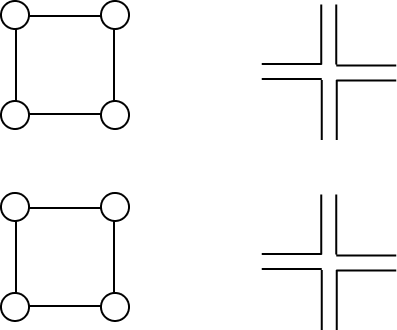
\includegraphics[width=0.79\linewidth,valign=t]{images/feynman-1.png}

        \vspace{5mm}
        
        \caption{$\Tr(\bA^4)^2$ represented as two squares in our notation, compared to the 't Hooft double line notation.}
        \label{fig:feynman-left}
    \end{subfigure}
    \hfill
    \begin{subfigure}[t]{0.45\linewidth}
        \centering
        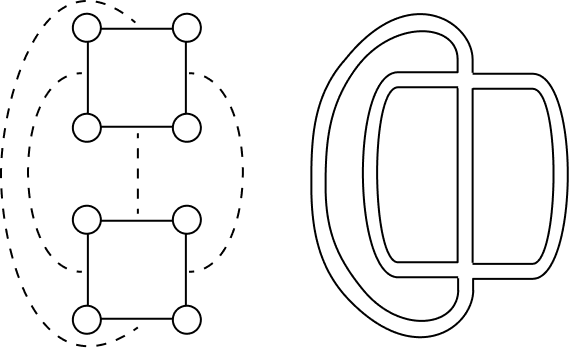
\includegraphics[width=\linewidth,valign=t]{images/feynman-2.png}

        \vspace{3mm}
        
        \caption{One of the Wick contractions appearing in $\langle \Tr(\bA^4)^2\rangle_\goe$. The edges of the squares are glued together according to the matching to make a ``pillow''.}
        \label{fig:feynman-right}
    \end{subfigure}

    \caption{Our Feynman diagram notation vs.\ the 't Hooft double line notation.}
    \label{fig:feynman-diagrams}
\end{figure}

The delta functions in the propagator enforce that the vertices of the squares have a consistent index $i$ when the edges of the squares are glued together.
Note that the propagator in~\cref{eq:propagator} for the \goe model allows $\bA[i,j], \bA[k,\ell]$ to be glued in either orientation (in contrast to the Gaussian Unitary Ensemble which would only have one term).
Therefore, we define a Feynman diagram for the \goe to be an \emph{oriented} perfect matching between the edges of the squares.
For each Feynman diagram $\gam$, the contribution of $\gam$ to~\cref{eq:taylor-exp} is:
\begin{enumerate}[(i)]
    \item a factor $n$ per vertex of $\gam$, since each vertex holds an index from $[n]$ which is summed over in $\Tr(\bA^4)$.
    \item a factor $\frac 1n$ per paired edge of $\gam$ from the propagator,~\cref{eq:propagator}.
    \item a factor $-\frac{gn}{8}$ per square face of $\gam$ from~\cref{eq:taylor-exp}. There is also an overall factor of $\frac{1}{|F(\gam)|!}$ where $|F(\gam)|$ equals the number of square faces in $\gam$.
\end{enumerate}

For example, the $s=1$ term in~\cref{eq:taylor-exp} is
\begin{equation*}
    \left(-\frac{gn}{8}\right)\cdot \langle \Tr(\bA^4)\rangle_\goe = \left(-\frac g 8\right) \cdot  \left(2\cdot n^2 + 5 \cdot n + 5 \right)\,.
\end{equation*}
The Feynman diagrams are enumerated in~\cref{fig:feynman-square}.

\begin{figure}[ht]
    \centering
    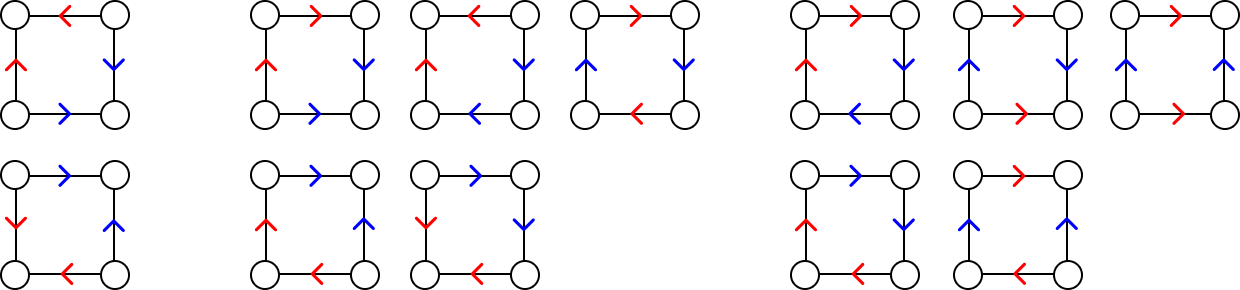
\includegraphics[width=0.9\linewidth]{images/feynman-square-alt.png}
    \caption{The 12 Feynman diagrams associated to $\langle \Tr(\bA^4)\rangle_\goe$. The two red edges are matched in the orientation specified by the arrows, and similarly for the blue edges. Gluing either of the left two diagrams results in a ``taco''. Gluing the remaining diagrams results in degenerate polyhedra. After gluing, the ``tacos'' have 3 vertices, the middle diagrams have 2 vertices, and the right diagrams have 1 vertex, respectively.}
    \label{fig:feynman-square}
\end{figure}

For a given Feynman diagram $\gam$, the total factor of $n$ is $|V(\gam)| - |E(\gam)| + |F(\gam)| =: \chi(\gam)$ which is the \emph{Euler characteristic} of the polyhedron $\gam$.
In total, we obtain a Feynman diagram expansion for the partition function,
\begin{equation}\label{eq:feynman-fml-1}
    Z = Z_{\goe} \sum_{\gam \in \Gam} \frac{1}{|F(\gam)|!}\left(-\frac{g}{8}\right)^{|F(\gam)|} n^{\chi(\gam)}\,,
\end{equation}
where $\Gam$ is the set of Feynman diagrams, the set of polyhedra built from square faces. Formally, $\Gam = \sqcup_{s \geq 0} \Gam_s$, where $\Gam_s$ is the set of oriented perfect matchings between the edges of $s$ squares.

Taking the logarithm has the effect of restricting the summation to \emph{connected} Feynman diagrams; this is the linked cluster theorem in quantum field theory~\cite[Section~3.5]{etingof2024mathematical}.
We obtain:
\begin{equation}\label{eq:feynman-free-energy}
    \ln \left(\frac Z {Z_\goe}\right) = \sum_{\gam \in \Gam_c} \frac{1}{|F(\gam)|!}\left(-\frac{g}{8}\right)^{|F(\gam)|} n^{\chi(\gam)}\,,
\end{equation}
where $\Gam_c \subseteq \Gam$ are connected Feynman diagrams.


\subsubsection{Asymptotic limit \texorpdfstring{$n \to \infty$}{n -> infty}}

As $n \to \infty$,~\cref{eq:feynman-free-energy} significantly simplifies because only the \emph{planar} diagrams survive, i.e.\ polyhedra $\gam$ with ``no holes,'' which have the maximum possible Euler characteristic among connected graphs ($\chi(\gam) = 2$).
This foundational observation goes back to 't~Hooft~\cite{tHooft1974planar}.\footnote{
    't~Hooft studies unitarily invariant matrix models instead of orthogonally
    invariant ones.
    He takes a further step by sending $g\to 0$ at the rate $\Theta(1/\sqrt{n})$, i.e., fixing $\lambda = g^2n$ to be constant. His claim is that $\lambda$ is the only parameter characterizing the physical properties of observables in the large-$n$ limit, and by taking $\lam \to \infty$ one gains some intuition on the physical phenomena of strongly interacting particles.
    The limit $g \to 0$ is less interesting for us, since the traffic distribution (hence also the spectrum) is asymptotically the same as the GUE whenever $g = o(1)$.
} We obtain, at first order,
\begin{equation}
    \frac{1}{n^2}\ln \left(\frac Z {Z_\goe}\right) = \sum_{\substack{\gam \in \Gam_c\\\text{planar}}} \frac{1}{|F(\gam)|!}\left(-\frac{g}{8}\right)^{|F(\gam)|} + O(n^{-2})\,.\label{eq:thooft}
\end{equation}

In summary,
the Feynman diagram method shows that the non-Gaussian component of the matrix model can be replaced by a
generating function for graphs/surfaces which, in the $n\to \infty$ limit,
restricts to a generating function for planar graphs/surfaces with genus 0.
This restriction leads to significant simplifications in diagrammatic calculations,
in the same way as our cactus property and treelike property in the rest of the paper.

\subsection{Calculation of general observables\texorpdfstring{: Argument for~\cref{thm:moments}}{}}

We now assume that the potential $V(\bA)$ has the general form $V(\bA)=\frac 12 \bA^2 + \sum_{j\geq 3}c_j\bA^j$ (arbitrary coefficients on $\bA$ and $\bA^2$ can be handled by centering and rescaling, respectively).
We compute the traffic distribution of $\bA$,
which consists of all $S_n$-invariant observables of $\bA$. The $z$-polynomials are a basis for these observables where, for each multigraph $\al$,
\begin{equation*}
    \frac 1n\langle z_\al(\bA) \rangle = \frac 1n \sum_{i : V(\al) \embeds [n]}\left\langle\prod_{\{u,v\} \in E(\al)} \bA[i(u), i(v)]\right\rangle\,.
\end{equation*}
Separating out the Gaussian part of the action from the higher-order interactions:
\begin{align*}
    \frac 1n\langle z_\al(\bA) \rangle = \frac 1n \cdot \frac{\left\langle z_\al(\bA) \exp(-\sum_{j \geq 3} c_j n \Tr(\bA^j)) \right\rangle_\goe}{\left\langle \exp(-\sum_{j \geq 3} c_j n \Tr(\bA^j)) \right\rangle_\goe}\,.
\end{align*}

The dual Feynman diagrams are built from polygons with $j\ge 3$ sides, each of which comes with a factor of $-c_j$, generalizing the situation from the previous section.
A small generalization of the argument
shows that the denominator is
\begin{equation}\label{eq:denom}
    \left\langle \exp(-\sum_{j \geq 3} c_j n \Tr(\bA^j)) \right\rangle_\goe = \sum_{\gam \in \Gam} \left(\prod_{j \geq 3} \frac{(-c_j)^{|F_j(\gam)|}}{|F_j(\gam)|!}\right) n^{\chi(\gam)}\,,
\end{equation}
where $|F_j(\gam)|$ denotes the number of $j$-sided faces in $\gam$.

The numerator can also be calculated diagrammatically.
The Wick contractions go between a collection of polygons as well as the additional edges $\bA[i,j]$ in $z_\al(\bA)$\,.
Let $\Gam(\al)$ be the set of Feynman diagrams, visualized as polyhedra built on a set of ``boundary'' edges $\al$.
Then

\begin{equation}\label{eq:num}
    \left\langle z_\al(\bA) \exp(-\sum_{j \geq 3} c_j n \Tr(\bA^j)) \right\rangle_\goe = \sum_{\gam \in \Gam(\al)} \left(\prod_{j \geq 3} \frac{(-c_j)^{|F_j(\gam)|}}{|F_j(\gam)|!}\right) n^{\chi(\gam)}\cdot(1-O(n^{-1}))\,.
\end{equation}

Note $\al$ is considered a boundary and does not count towards the faces $F_j(\gam)$.

To enforce that the labels of $z_\al(\bA)$ are injective, we remove from $\Gam(\al)$ any matching which causes two vertices of $\al$ to have the same label.
The factor $1-O(n^{-1})$ arises because each vertex is summed over $n - O(1)$ indices to maintain injectivity, instead of precisely $n$ which we had previously.

We obtain the final result by
dividing~\cref{eq:num} by~\cref{eq:denom}.
This has the effect of restricting to the set of connected Feynman diagrams $\Gam_c(\al) \subseteq \Gam(\al)$ by an alternate version of the linked cluster theorem.
The final Feynman diagram formula is:
\begin{align}
    \frac 1n \langle z_\al(\bA)\rangle &= \sum_{\gam \in \Gam_c(\al)} \left(\prod_{j \geq 3}\frac{\left(-c_j\right)^{|F_j(\gam)|}}{|F_j(\gam)|!} \right) \cdot n^{\chi(\gam)-1}\cdot(1-O(n^{-1}))\,. \label{eq:feynman-alpha}
\end{align}

\begin{remark}
An alternative approach to the calculation would be to first symmetrize $z_\al(\bA)$ over $O(n)$ 
which is the symmetry group of the matrix model (and is larger than $S_n$),
then to plug in the values of the $O(n)$-invariant observables (the trace polynomials).
We find it simpler to Taylor expand the action directly.
\end{remark}

\subsubsection{Asymptotic limit \texorpdfstring{$n\to\infty$}{n -> infty}}

In the asymptotic limit $n \to \infty$,
the only diagrams in~\cref{eq:feynman-alpha} with constant-order magnitude are those such that $\al$ is a cactus graph, and $\gam$ consists of polyhedra with genus 0 attached to each cycle of the cactus, which has $\chi(\gam) = 1$.
We prove this combinatorially in the forthcoming~\cref{lem:combinatorially-dominant}.

The large-$n$ combinatorial summation factors over the cycles of the cactus, since the genus-0 polyhedra on each cycle can be chosen independently.
We obtain
\begin{equation*}
    \frac 1n \langle z_\al(\bA) \rangle = \begin{cases}
        \displaystyle\prod_{\sig \in \cycles(\al)} \frac 1n \langle z_\sig(\bA)\rangle  + O(n^{-1}) &\text{ if $\al$ is a cactus}\\
        O(n^{-1}) & \text{otherwise}
    \end{cases}
\end{equation*}
The limiting value $\frac 1n \langle z_\sig(\bA)\rangle$ of the $q$-cycle diagram $\sig$ is equal to $\kappa_{q} + O(n^{-1})$ by the moment/free cumulant relation~\cref{eq:freeCumulantRelation}. Thus,~\cref{eq:feynman-alpha} recovers~\cref{thm:moments}.


\begin{lemma}\label{lem:combinatorially-dominant}
    Let $\al \in \calA$ be a connected multigraph, and let $\gam \in \Gam_c(\al)$.
    Then $\chi(\gam) = 1$ if and only if $\al$ is a cactus and $\gam$ consists of genus-0 polyhedra attached to each cycle of $\al$.
\end{lemma}
\begin{proof}
The only $\al$ for which $\Gam_c(\al)$ is nonzero are the Eulerian $\al$,
since a polyhedron $\gam \in \Gam_c(\al)$ with boundary $\al$ must have a boundary which is a union of cycles.
Therefore, it remains to argue about Eulerian graphs $\al$.

For Eulerian $\al$, the $\gam \in \Gam_c(\al)$ which maximize the quantity $\chi(\gam) = |V(\gam)| - |E(\gam)| + |F(\gam)|$ are given by decomposing $\al$ into the maximum number of simple cycles, then attaching a genus 0 polyhedron to each cycle.
This achieves $\chi(\gam) = |V(\al)| - |E(\al)| + C$ where $C$ is the number of cycles.\footnote{Note that the computational problem of, given an Eulerian graph $\al$, compute a partition of $E(\al)$ into the maximum number of cycles, is NP-hard \cite{Holyer81:EdgePartitioning}.}

We argue that:
\begin{equation}\label{eq:max-cycle-partition}
    |V(\al)| - |E(\al)| + C \leq 1
\end{equation}
for all Eulerian graphs $\al$ and this is achieved if and only if $\al$ is a cactus.
Fix a maximum cycle partition of $\al$. The $C$ cycles are edge-disjoint so we can remove one edge from each one while maintaining that the graph is connected. Let $\al'$ be the resulting graph. Then $|V(\al')| - |E(\al')| = |V(\al)| - |E(\al)| + C$. Since $\al'$ is still connected we have $|V(\al')| - |E(\al')| \leq 1$.
The final inequality is an equality if and only if $\al'$ is a tree and hence $\al$ is a cactus.
This proves~\cref{eq:max-cycle-partition} and completes the lemma.
\end{proof}



\subsection{Mathematical comments on the Feynman diagram method}
\label{app:feynman-formal}

The Feynman diagram method is not mathematically rigorous, with (in our opinion)
the main obstruction being that intermediate summations such as~\cref{eq:feynman-fml-1,eq:num,eq:feynman-free-energy} are divergent.
The Euler characteristic grows with the
number of disconnected polyhedra, but the method proceeds anyway to divide out the disconnected polyhedra,
which ultimately yields a convergent summation in~\cref{eq:thooft} (for sufficiently small values of the coupling constant $g \geq 0$).


The Feynman diagram method is a {perturbative expansion}
because it holds for sufficiently small perturbations of the \goe density,
up to the radius of convergence of the Feynman diagram summations~\cite{mcLaughlin,garouf}.
On the other hand,~\cref{thm:moments} holds beyond the radius of convergence of the Feynman diagram expansion in~\cref{eq:feynman-alpha},
so it would be impossible to prove the theorem using a perturbative expansion alone.